\section{Post-Training}
\label{sec:alignment}



We follow the same general recipe as Nemotron 3 Nano, with a stronger emphasis on agentic tasks. Figure~\ref{fig:posttraining_stages} provides an overview of the pipeline. We begin with a Supervised Fine-Tuning (SFT) phase (\S\ref{subsec:SFT}), followed by a three-stage Reinforcement Learning phase—RLVR, SWE-RL, and RLHF (\S\ref{subsec:RL}). We conclude with a final phase of MTP healing.

In SFT, we expand the training blend to cover a wider range of agentic harnesses and interaction scenarios. We also significantly improved our RL infrastructure, enabling reliable large-scale asynchronous training on thousands of GPUs. This infrastructure allows us to (1) train across 21 diverse environments, improving robustness across tasks, and (2) train on long-horizon SWE tasks, strengthening multi-step reasoning and problem solving in realistic agentic settings.
% \todo{Jian should update what would be the section and assign the appropriate people to contribute}

\begin{figure}[h]
    \centering
    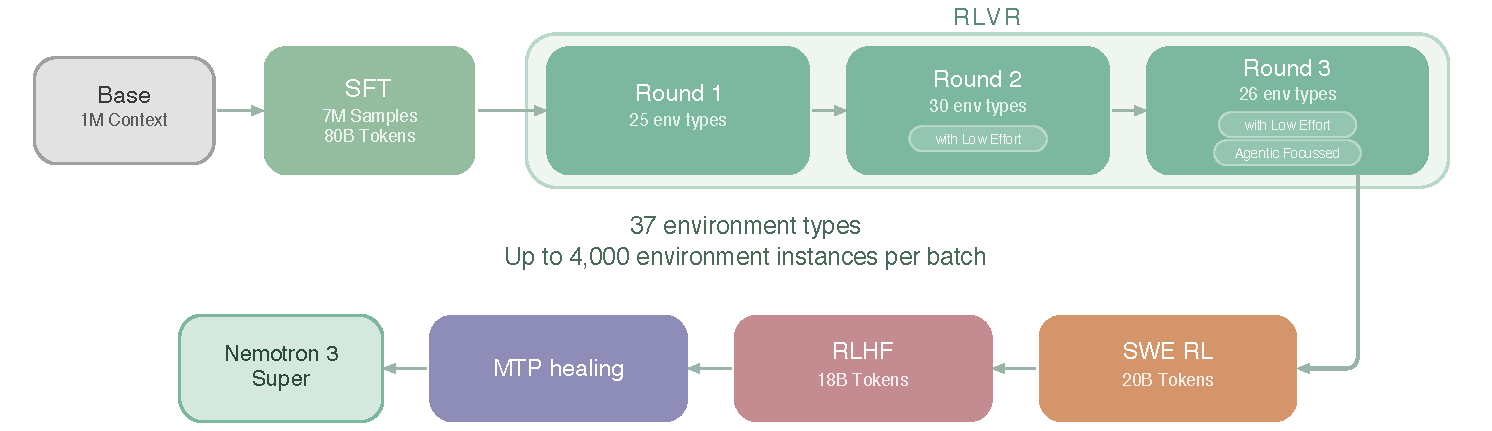
\includegraphics[width=\linewidth]{figures/posttraining-stages.pdf}
    \vspace{-0.5em}
    \caption{Overview of the post-training pipeline for \ourmodel.}
    \label{fig:posttraining_stages}
    \vspace{-0.5em}
\end{figure}

\subsection{Supervised Fine Tuning}
\label{subsec:SFT}
For \ourmodel SFT, we focused on improving dataset quality and diversity. In particular, we scaled up our agentic datasets and increased their share in the overall SFT blend. The chat template remains identical to \nanomodel. In addition, we add low effort reasoning mode, giving users further control over reasoning length. We found that a single-stage SFT led to a marked degradation on long-input-short-output scenarios. We therefore adopt a two-stage SFT procedure: Stage~1 emphasizes learning from token-level supervision and induces strong reasoning behavior, while Stage~2 switches to per-conversation normalization to prevent long outputs from dominating the loss, which restores long-input-short-output performance while retaining reasoning. We describe it below:

\subsubsection*{SFT objective and two-stage loss}

% We supervise the model only on \emph{output} (assistant) tokens, masking prompt tokens.
For a packed global batch $\mathcal{B}$ containing multiple conversations $c$, let $\mathcal{O}_c$ denote the set of output-token positions for conversation $c$ and $|\mathcal{O}_c|$ its output-token count. With token-level negative log-likelihood $\ell_t = -\log p_\theta(y_t \mid x, y_{<t})$, we use:

\paragraph{Stage 1: token-level (global) average.}
We minimize the average loss over \emph{all} output tokens in the packed global batch:
\begin{equation}
\mathcal{L}_{\text{tok}}
= \frac{\sum\limits_{c \in \mathcal{B}} \sum\limits_{t \in \mathcal{O}_c} \ell_t}
{\sum\limits_{c \in \mathcal{B}} |\mathcal{O}_c|}.
\end{equation}
This corresponds to summing the output-token log probabilities across all conversations and normalizing by the total number of output tokens.


\paragraph{Stage 2: sample-level average.}
We then switch to a per-conversation normalized loss and average equally across conversations:
\begin{equation}
\mathcal{L}_{\text{samp}}
= \frac{1}{|\mathcal{B}|} \sum\limits_{c \in \mathcal{B}}
\left(
\frac{1}{|\mathcal{O}_c|} \sum\limits_{t \in \mathcal{O}_c} \ell_t
\right).
\end{equation}
This stage reduces the dominance of long outputs by normalizing each conversation by its own output-token count before averaging across the batch.

For Stage 1, we run SFT with 256k sequence length packing, global batch size 64, constant lr $1e-5$ with 30k warmup samples.
 For Stage 2, we use 512k sequence length packing and include long context data with length up to 512K, global batch size 32 and constant lr $1e-5$. 

\paragraph{MTP during SFT} We continue training \ourmodel with the same shared-weight MTP head used in pretraining to preserve both the accuracy benefits of multi-step prediction and the inference-time gains from speculative decoding. Concretely, we train two MTP layers with shared parameters and optimize the combined objective using a scaled auxiliary loss computed with per-token loss and 0.3 scaling factor. 


\subsubsection{Data}

We reuse the following datasets from the \nanomodel SFT datasets: Chat, Infinibyte,  and Formal Proofs. We refresh the following datasets with new teacher models (\texttt{DeepSeek v3.2, Kimi K2}): Competition Math, Competition Code,  Conversational Tool Use, Multilingual, Science. Below we describe new or heavily modified SFT datasets.

\textbf{Software Engineering.}
We curate a dataset of coding tasks derived from real-world GitHub issues to train \ourmodel for autonomous software engineering capabilities including code exploration, task tracking, issue reproduction and bug fixing. We use the issues and containerized execution environments from the SWE-Gym \citep{pan2025trainingsoftwareengineeringagents}, R2E-Gym \citep{jain2025r2egymproceduralenvironmentshybrid} and SWE-rebench \citep{badertdinov2025swerebenchautomatedpipelinetask} datasets. For R2E-Gym, we regenerate problem statements with \texttt{Qwen3-Coder-480B-A35B-Instruct}. We distill trajectories from the OpenHands agent harness using \texttt{Qwen3-Coder-480B-A35B-Instruct} as the teacher model.

\textbf{Agentic Programming.}

\begin{figure}[t!]
    \centering
    % \includegraphics[width=\textwidth]{figures/agentic_pipeline.png}
    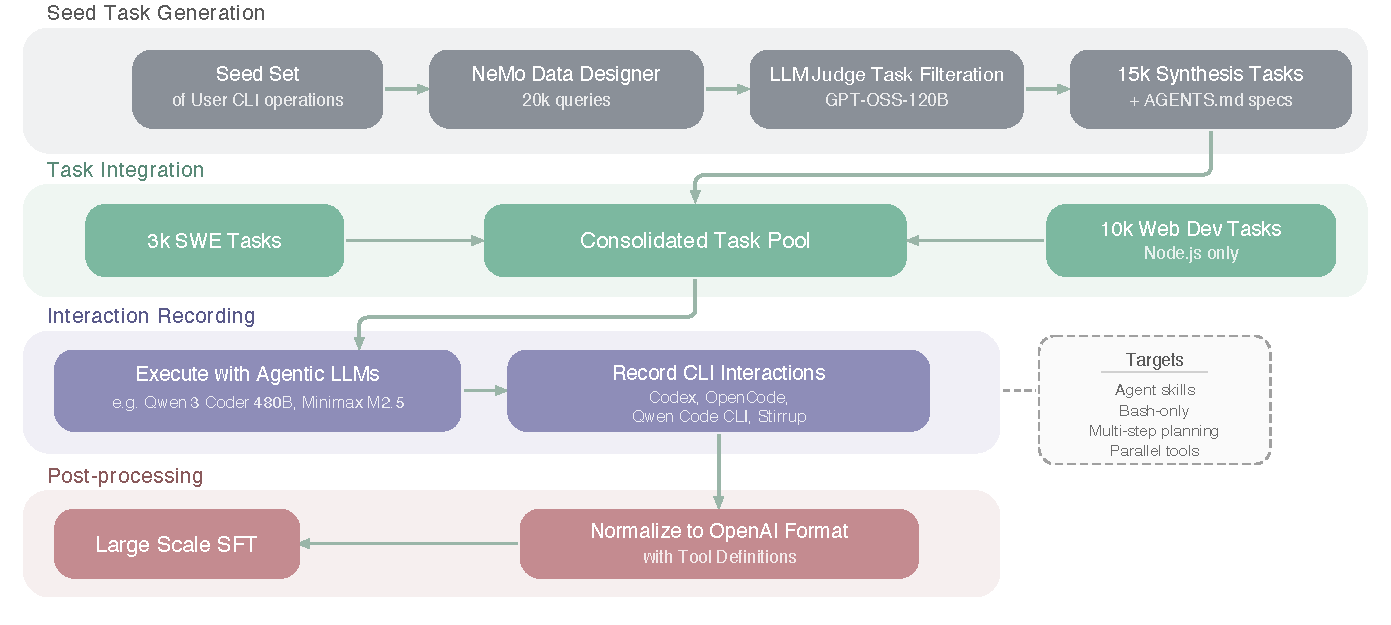
\includegraphics[width=\textwidth]{figures/swe-sft-data.pdf}
    \vspace{-1em} % Adjust spacing between image and text
    \caption{Agentic Command Line Interface Dataset Construction \& Training Pipeline}
    \label{figure:agentic_data_pipeline}
\end{figure}
% 
The landscape of software development has undergone a substantial shift with the emergence of Agentic Command Line Interface (CLI) tools, moving beyond the "autocomplete" era of 2021–2023 into a regime of autonomous execution. Alongside substantial improvements in harnesses such as Claude Code, OpenCode, and OpenAI’s Codex, models are now capable of operating as active digital collaborators, capable of multi-step reasoning, long-horizon execution, and end-to-end task orchestration. 

We established a foundational seed set of tasks designed to replicate common user-initiated operations within agentic CLIs. Refer to Figure \ref{figure:agentic_data_pipeline} where we discuss the full pipeline. We utilized NeMo Data Designer \citep{nemo-data-designer} to generate approximately 20k queries derived from a taxonomy of 24 distinct actions typically performed in these environments. Subsequently, we employed \texttt{GPT-OSS 120B} \citep{openai2025gptoss120bgptoss20bmodel} in an LLM-as-a-Judge framework to filter out tasks referencing pre-existing codebases or modifications to extant files. This mitigation ensures that the models do not attempt modification operations within empty directories—a scenario that frequently results in redundant and exhausted tool invocations during failed execution cycles. The resulting dataset comprises roughly 15k tasks centered on direct solution synthesis. To further enhance the diversity of the generated outputs, we coupled each task with a supplementary markdown specification, equivalent to an AGENTS.md file. These documents impose additional constraints and architectural requirements, effectively narrowing the design space and necessitating more complex, varied solutions from the agent.

Since we eliminate all tasks that require a pre-existing codebases, we augment this task set with roughly 3000 questions from SWE tasks that are challenging and come with pre-existing repository and specific git hash commit. We apply a simple prompt prior to the existing issue statements, stating that the execution environment does not have the library installed and therefore execution of unit tests should be avoided. This is a conscientious decision made to substantially reduce the engineering effort required to support per sample container based execution of each SWE task, reduce the number of tool calls and avoid large tool outputs due to multiple rounds of unit test executions. This further relaxes the constraints imposed on the agent to solve the issue, as there is no SWE specific prompt to guide the agent in solving the task. Finally, we synthesize 10k web development tasks using a taxonomy of 100 fine-grained tasks that are commonly requested by users as the seed, on which we apply LLM-as-a-Judge to eliminate tasks that require a pre-existing repository. We impose no restrictions on these tasks, but provide only a Node.js environment and expect the agent to setup and install all dependencies and plugins on its own.

Applying these task sets, we distill from high-performance, open-source agentic LLMs such as \texttt{Qwen-3-Coder-480B} \citep{qwen2025qwen25technicalreport} and \texttt{Minimax M2.5} \citep{minimax2025m2} by recording their interactions with various CLI environments, such as Codex, OpenCode, Qwen Code CLI, and Stirrup. These interaction traces are subsequently filtered, normalized into the standard OpenAI message format with various tool definitions, and utilized for large-scale SFT to effectively embed agentic operational knowledge within the model. For each Agentic CLI, we study the individual capabilities that exist and are commonly utilized. We apply the same task sets to target different capabilities, such as Agent Skills, tool restriction (bash only execution), ask user clarifying questions, single and multi step planning, static and dynamic multi turn conversations and parallel tool calling, depending on whether the specific CLI can accommodate these capabilities. 

\textbf{Long Context.}
We extend the long-context SFT dataset from \nanomodel with a more comprehensive synthetic data pipeline. To improve long-context multi-document reasoning, we construct a synthetic SFT dataset using long sequences from our pre-training blend, which contains books, papers, financial reports, code repositories, etc. We first cluster these documents by topic/domain and concatenate related documents to reach target sequence lengths, such as 128K, 256K, or 512K tokens. 
% Optionally, we use shorter excerpts (e.g., 128K if the target sequence length is 512K) during synthetic data generation while retaining the full concatenated context during SFT. 
For each long-context sample, we use an LLM to generate one or more QA pairs. The prompt requires questions to involve cross-document or cross-section navigation, ensuring information is scattered rather than localized. It strictly enforces multi-hop reasoning, requiring at least 4 to 7 distinct retrieval or reasoning steps. These steps mandate computational or logical processing, preventing simple copy-pasting, and often include explicit formatting instructions. Next, we generate 8 independent reasoning traces for each context-question pair. We apply semantic majority voting to group the answers, either by exact match or via an LLM judge. From the resulting majority group, we select the answer containing the shortest reasoning trace. 
% Finally, to ensure the dataset provides a meaningful learning signal, we apply difficulty filtering by having the target model evaluate the samples. Any instances that the target model can already answer correctly prior to fine-tuning are discarded. Throughout this pipeline, we utilize \texttt{Qwen3-235B-A22B-Thinking-2507} \citep{yang2025qwen3technicalreport} for QA generation, reasoning trace generation, and semantic majority voting. For the final difficulty filtering step, we employ \texttt{Qwen3-235B-A22B-Instruct-2507} \citep{yang2025qwen3technicalreport} as the judge. 
Additionally, we generate seven synthetic reasoning tasks to improve the model's ability to process context in a sequential, left-to-right manner. Specifically, synthetic snippets (generated using \texttt{Qwen3-235B-A22B-Thinking-2507}) are concatenated together to form long input context. The thinking traces are constructed by chaining rule-based reasoning steps, each of which includes relevant excerpts from the input context and tracking metadata, such as the frequency of query-related snippets.
%We also construct input context upto required length by concatenating records from ~\cite{nvidia/Nemotron-Personas-USA} and prepare questions emphasizing multi-hop reasoning and information aggregation. Context, question and answers are formatted via pre-defined templates and ground truth is derived by running sql queries on records.
We also construct long-context samples by concatenating records from~\citep{nvidia/Nemotron-Personas-USA} to reach the required sequence length. Questions are designed to emphasize multi-hop reasoning and information aggregation across records. Context, question, and answer are formatted using pre-defined templates, with ground-truth answers derived by executing SQL queries over the underlying records.

\textbf{Financial Reasoning.}
To construct a large-scale training corpus for financial reasoning, we employ a template-based synthetic data generation (SDG) pipeline that scales a curated seed set into hundreds of thousands of grounded question--answer pairs. The pipeline sources 565 expert-authored seed questions from the SecQue benchmark~\citep{benyoash2025secque}, a dataset of financial analysis questions anchored to SEC 10-K and 10-Q filings. These seeds are expanded combinatorially across S\&P~500 companies\footnote{\url{https://en.wikipedia.org/wiki/List_of_S\%26P_500_companies}, accessed 2025.} and fiscal years (2019--2024), where comparative questions are restricted to company pairs within the same GICS Sub-Industry to preserve semantic coherence. GPT-OSS-120B paraphrases each template instantiation, producing up to three diverse reformulations per combination. The resulting questions are mapped to relevant SEC filing sections using the original SecQue metadata, and the corresponding documents are converted to markdown with a configurable token limit. For answer generation, we adopt the GenSelect strategy~\citep{toshniwal2025genselectgenerativeapproachbestofn}: five candidate answers are sampled per question using GPT-OSS-120B with distinct random seeds, and a larger judge model (Qwen3-235B-A22B) selects the best response based on numerical accuracy, financial methodology, and logical soundness. A smaller model (Qwen3-30B-A3B) then classifies each pair as \texttt{ANSWERABLE} or \texttt{UNANSWERABLE}, retaining only those containing a complete, substantive response. Prior to supervised fine-tuning, the SDG output undergoes percentile-based outlier removal and deduplication. The resulting dataset comprises 366,243 financial Q\&A pairs with reasoning traces.

\textbf{CUDA.}
A large-scale synthetic CUDA dataset comprising 100K samples for kernel generation, repair, and optimization was constructed using a synthetic data generation pipeline based on \texttt{DeepSeek-R1} and \texttt{GPT-OSS-120B}. Seed questions were sourced from popular open-source libraries, NVIDIA library API surfaces, and BackendBench \citep{saroufim2025backendbench}. These seeds were used to generate tuples of the form (PyTorch reference, CUDA C++ kernel) and (natural language specification, CUDA C++ kernel), each accompanied by reasoning. For each seed item, multiple candidate kernels were generated and rigorously validated for correctness within an internal CUDA evaluation environment. The validated kernels were then ranked by performance, and the highest-performing kernel was retained. In addition, we collected traces from an internal CUDA agent, producing samples of the form (PyTorch reference, faulty CUDA C++ kernel, error message, corrected CUDA C++ kernel) and (PyTorch reference, slow CUDA C++ kernel, Nsight Compute log, optimized CUDA C++ kernel). Using publicly available documentation and official code samples, and following the same formulation as the CUDA-C data, we generated additional PyTorch references and corresponding CUDA-library implementations with reasoning chains, as well as aligned natural language specifications. These libraries include Thrust, CUB, cuBLAS, cuDNN, cuSPARSE, cuRAND, and cuSOLVER.

% NOTE, Prasoon: I shortened it even further from our already shortened version, but we've something brand new in the SDG generation method so need some space to explain., @soumye/@alex if you feel there is need to still shorten more, please reach out to me/Makesh again.
\textbf{Safety.} We have significantly enhanced our safety framework compared to \nanomodel by combining a robust prompt library with a two-stage synthetic response generation strategy. While retaining the core prompts from Nemotron Content Safety v2 \citep{ghosh-etal-2025-aegis2}, Gretel Safety Alignment v1 \citep{gretelai_gretel-safety-alignment-en-v1}, Harmful Tasks \citep{hasan2024pruning} and Red-Team-2K \citep{luo2024jailbreakv_robustness} covering content safety and common jailbreak techniques, we added in new synthetic prompts targeting the elicitation of over-refusals, demographic biases, and copyright reproduction. We also expand coverage of jailbreak strategies to better capture emerging adversarial techniques including indirect prompt injection attacks. 

Our primary advancement over \nanomodel is an explicit response policy framework. For each prompt, a response policy is inferred from a combination of prompt metadata, its annotated safety category, and predictions from a set of lightweight auxiliary classifiers that detect attributes such as self-harm risk, demographic targeting, or the presence of embedded adversarial instructions. We cast this decision process as a multi-class classification problem, where each class corresponds to a distinct response mode aligned with safety guidelines. These response modes specify whether the model should provide supportive resources such as helpline information, issue a refusal with a brief explanation, or answer the benign portion of the request while ignoring malicious content. This ensures that the responses are safe, contextually appropriate, and consistent across a diverse set of safety-sensitive scenarios.

Following the deliberative alignment framework \citep{guan2025deliberativealignmentreasoningenables}, we adopt a two-stage generation process in which the reasoning trace and the final response are curated separately but consistently with our response policy. In the first stage, we construct a concise reasoning trace that guides the model to reflect on the safety properties of the prompt, explicitly identifying why the request may be unsafe or policy-relevant and what constraints should govern the response. In the second stage, we generate the final response based on this reasoning trace, ensuring that it adheres to the predefined response policy and behavior guidelines. This structured separation encourages deliberate reflection on safety guidelines while producing responses that are consistent, policy-compliant, and contextually appropriate to ensure that the final response follows safety policies while minimizing unnecessary references to said policies. Finally, we apply a content-moderation classifier to filter any responses flagged as unsafe, providing an additional safeguard to ensure alignment with safety objectives.

\textbf{Search.}
To improve search capabilities, we generated a synthetic search-agent SFT dataset using NeMo Data Designer \citep{nemo-data-designer}. The pipeline begins by constructing seed prompts grounded in the Wikidata knowledge graph \citep{vrandecic2014wikidata}: we query SPARQL \citep{sparql2013} for well-connected hub entities across approximately 25 verified entity classes (cities, universities, films, chemical elements, etc.), then perform random walks of 4-8 hops through the graph, filtering out degenerate paths via stop-node lists, anti-meta-relation exclusions, and minimum path-length thresholds. Each valid walk yields a start entity, a chain of factual relations, and a final answer entity.

Data Designer then processes these seeds in three stages: (1) a draft stage converts the structured knowledge-graph walk into a natural-language multi-hop question, (2) an obfuscation stage rewrites the question to hide intermediate entities and eliminate breadcrumb-style chaining -- producing search-riddle queries where the solver must decompose the problem independently -- and (3) an agent stage in which MiniMax-M2 \citep{minimax2025m2} solves the obfuscated question by issuing web searches via the Tavily (\url{https://tavily.com}) MCP search tool, producing a grounded search trajectory with supporting URLs. Each resulting SFT record is a multi-turn conversation where assistant turns interleave chain-of-thought reasoning with structured tool calls, and tool-response turns return search results as JSON, preserving a full Thought--Action--Observation loop across an average of 12 tool calls per trajectory. A final structured-output stage normalizes the agent's raw response into a validated JSON schema. 
% Pre-generation filters remove seeds with generic or abstract answer entities, and post-generation validators discard samples lacking tool calls, supporting URLs, or substantive justifications, yielding approximately 7K training records.


\textbf{Terminal Use.}
The dataset for enhancing terminal capabilities follows the dual-stream \textit{Terminal-Task-Gen} methodology described in Nemotron-Terminal \citep{pi2026dataengineeringscalingllm}, comprising a total of 84,864 samples. This pipeline combines the adaptation of existing high-quality datasets with synthetic task generation grounded in a comprehensive terminal skill taxonomy. The source distribution consists of 68,924 synthetic samples, 8,125 samples from Nemotron-Cascade-Math, and 7,815 samples from Nemotron-Cascade-Code \citep{wang2025nemotroncascadescalingcascadedreinforcement}. For trajectory construction, we use \texttt{DeepSeek-V3.2} \citep{deepseekai2024deepseekv32} as the primary engine to generate step-by-step solution traces within isolated, Dockerized environments through an agentic execution-feedback loop. All samples are generated using the Terminus 2 agent framework~\citep{merrill2026terminalbenchbenchmarkingagentshard} as the underlying scaffolding, providing a unified set of terminal tools and a structured interaction protocol to maintain consistency and quality across long-horizon trajectories.

\textbf{Multilingual.}
Our multilingual data combines synthetic translations of English SFT examples with a sentence-level parallel corpus to improve machine translation. We reuse the line-by-line translation pipeline from \nanomodel, translating into six languages (German, Spanish, French, Italian, Japanese, and Chinese) using \texttt{Qwen2.5-Instruct-14b}. After translation, we apply filtering to remove samples in the wrong language and other common failure modes. We observed a recurring pattern where translation disrupts the alignment between prompt specifications and answer formats — a consistency usually maintained in English data. This mismatch led to instruction-following failures during preliminary testing. To mitigate this, we introduced a lightweight post-editing step with \texttt{Qwen3-4B-Thinking-2507} to automatically restore format compliance. We also expand the parallel corpus with additional Chinese $\leftrightarrow$ English pairs and exclude very short samples that previously degraded post-training performance.


\textbf{Structured Query Language (SQL).}
To improve \ourmodel on enterprise SQL workloads, we generate a synthetic text-to-SQL dataset with NeMo Data Designer \citep{nemo-data-designer}. The dataset contains 96.5k records spanning MySQL, PostgreSQL, and SQLite across 60 industry sectors, $\sim$700 domain topics, and 90 SQL concept buckets (from basic SELECT to recursive CTEs, window functions, and geospatial queries). Each sample pairs a natural-language prompt and a fully synthetic database schema context with a target SQL query. To improve robustness and to mimic the real-world messiness of production databases, the pipeline injects distractor tables and columns into the database context. Specifically, related but irrelevant tables and columns are added to the database context, forcing the model to learn to ignore irrelevant schema elements. Prompt diversity is controlled along three axes -- instruction style (imperative, declarative, interrogative, contextual, abbreviated), linguistic register (formal, conversational, technical, academic, direct), and politeness level -- yielding naturalistic and varied user requests. The final dataset of 96.5k records is validated and filtered down by Data Designer from a larger dataset using per-dialect syntax validators and five LLM-as-a-critic judges.

% \textbf{Conversational Tool Use.} Creating a large set of broad and specialized tool-use data for training has been adopted into many models to boost agentic capabilities \citep{Liu2024ToolACE,deepseekai2024deepseekv32,kimiteam2025kimik2openagentic,5team2025glm45agenticreasoningcoding}. For \ourmodel, we scale the conversational tool use data by creating a fully synthetic, 6-stage data generation pipeline.
% \begin{enumerate}
%     \item Domain Generation: We sample multiple synthetic domains using a model, iteratively asking the model to build upon it's initial generation to further sample specialized subdomains.
%     \item Policy and Tool Generation: We use a model to sample various customer-service policies and related tools an agent can use, iteratively improving the sampled policies and tools using self-refinement. To maintain policy style and formatting, we use a few-shot prompt and utilize LM-as-a-Judge to filter for quality.
%     \item Scenario Generation: We use a model to generate a set of plausible user personas, background information, and inquiries for each policy setting.
%     \item Trajectory Collection: Using the policy and scenario pairs, we conduct $16$ customer service interactions between a model-simulated agent, user, and environment using the policy and scenario pairs.
%     \item Verification: We judge the quality of each trajectory in both the outcome and process level using LM-as-a-Judge.
%     \item SFT Data Selection: We choose successful trajectories for SFT training, filtering for difficulty by dropping all scenarios that resulted in all-success or all-failure.
% \end{enumerate}

\textbf{Conversational Tool Use.} Large-scale specialized tool-use training data has been adopted by many models to boost agentic capabilities \citep{Liu2024ToolACE,deepseekai2024deepseekv32,kimiteam2025kimik2openagentic,5team2025glm45agenticreasoningcoding}. For \ourmodel, we scale conversational tool-use data via a fully synthetic, six-stage generation pipeline:
\vspace{-0.25\baselineskip}
\begin{enumerate}
\item Domain Generation: Sample synthetic domains with a model, iteratively expanding initial generations into specialized subdomains.
\item Policy and Tool Generation: Sample customer-service policies and related tools, iteratively improving them via self-refinement; use few-shot prompting and an LM-as-a-Judge for quality filtering to maintain style and formatting.
\item Scenario Generation: Generate plausible user personas, background information, and inquiries for each policy setting.
\item Trajectory Collection: For each policy–scenario pair, simulate $16$ customer service interactions among a model-based agent, user, and environment.
\item Verification: Evaluate trajectories at both outcome and process levels using an LM-as-a-Judge.
\item SFT Data Selection: Select successful trajectories for SFT and filter for difficulty by dropping scenarios that yield all-success or all-failure outcomes.
\end{enumerate}

\begin{figure}[!t]
\centering
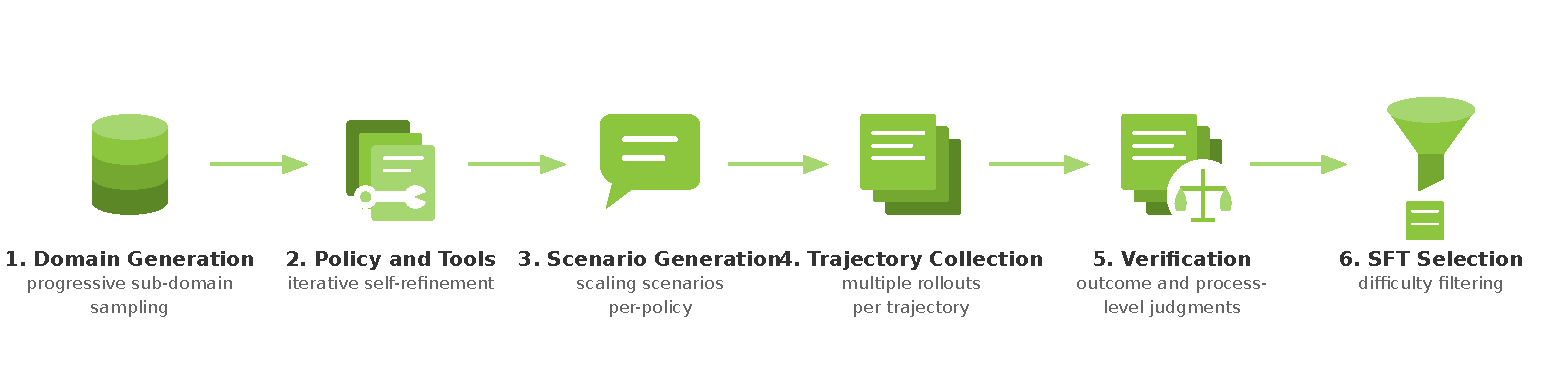
\includegraphics[width=0.9\linewidth]{figures/conversational_tool_use_data_generation.pdf}
\caption{Overview of the synthetic data generation pipeline for specialized conversational tool-use SFT data used for \ourmodel.}

\label{fig:conversational_tool_use_data_generation_pipeline}
\end{figure}


A visualization of the pipeline is shown in Figure \ref{fig:conversational_tool_use_data_generation_pipeline}. We utilize \texttt{Qwen3-235B-A22B-Thinking-2507}, \texttt{Qwen3-32B}, \texttt{Qwen3-235B-A22B-Instruct-2507} \citep{yang2025qwen3technicalreport}, \texttt{deepseek-r1-0528} \citep{deepseekai2025deepseekr1incentivizingreasoningcapability}, \texttt{DeepSeek-V3.2} \citep{deepseekai2024deepseekv32}, and \texttt{gpt-oss-120b} \citep{openai2025gptoss120bgptoss20bmodel} on various parts of the above pipeline, yielding 279{,}116 conversations across 838 domains. This represents a substantial scale-up over \nanomodel, which used 15{,}588 conversations spanning 5 domains.


\textbf{General-Purpose Tool Use.}
The broader, general purpose tool-calling synthetic data pipeline begins with the construction of diverse tool sets from ToolEyes \citep{ToolEyes2025}, API-Bank \citep{APIBank2023}, UltraTools \citep{Huang2024UltraTool}, AutoTools \citep{Shi2025AutoTools}, xLAM \citep{Zhang2024xLAM}, Glaive-Function-Calling-v2 \citep{GlaiveFunctionCallingV22025}, Toucan-1.5M \citep{Xu2025Toucan}, as well as custom written tools that serve as the foundation for downstream synthetic task generation. A tool-calling trajectory is simulated by grounding in one or multiple of these tool sets. The trajectory simulation involves an LLM playing three roles - User (User-LLM), Assistant (Assistant-LLM), and Tool Environment (Tool-LLM). The User-LLM is seeded with the selected tool set, a persona sampled from Nemotron-Personas-USA \citep{nvidia/Nemotron-Personas-USA}, and a tool-calling scenario (single-turn, multi-turn, or multi-step). The User-LLM starts by designing a task guided by the tool-calling scenario which is relevant to the selected persona and can be solved by the selected tool set. The Assistant-LLM attempts to solve this task in one or more turns by producing tool-calls and responding to tool execution results. The Tool-LLM is responsible for producing a simulated tool execution result based on the tool-call generated by the Assistant-LLM and the tool being called. The Tool-LLM is prompted with a rubric that helps identify syntactic and semantic errors in tool-calling, as well as the original user query so that the tool results can be contextualized when tool-call is successful. To ensure accuracy, we employ a turn-level and trajectory-level judge similar to the specialized tool-calling data generation. The turn level judge is also paired with a rule-based verification for ensuring correctness of tool-calls. We scale this pipeline with DeepSeek-v3.2 \citep{DeepSeekV32025} and GLM-4.7 \citep{GLM47Zai2025} to create a dataset of 1.5M diverse tool-calling trajectories.

The overall general-purpose synthetic tool-calling data pipeline is visualized in figure \ref{fig:broad_conversational_tool_use_data_generation_pipeline}.

\begin{figure}[!t]
\centering
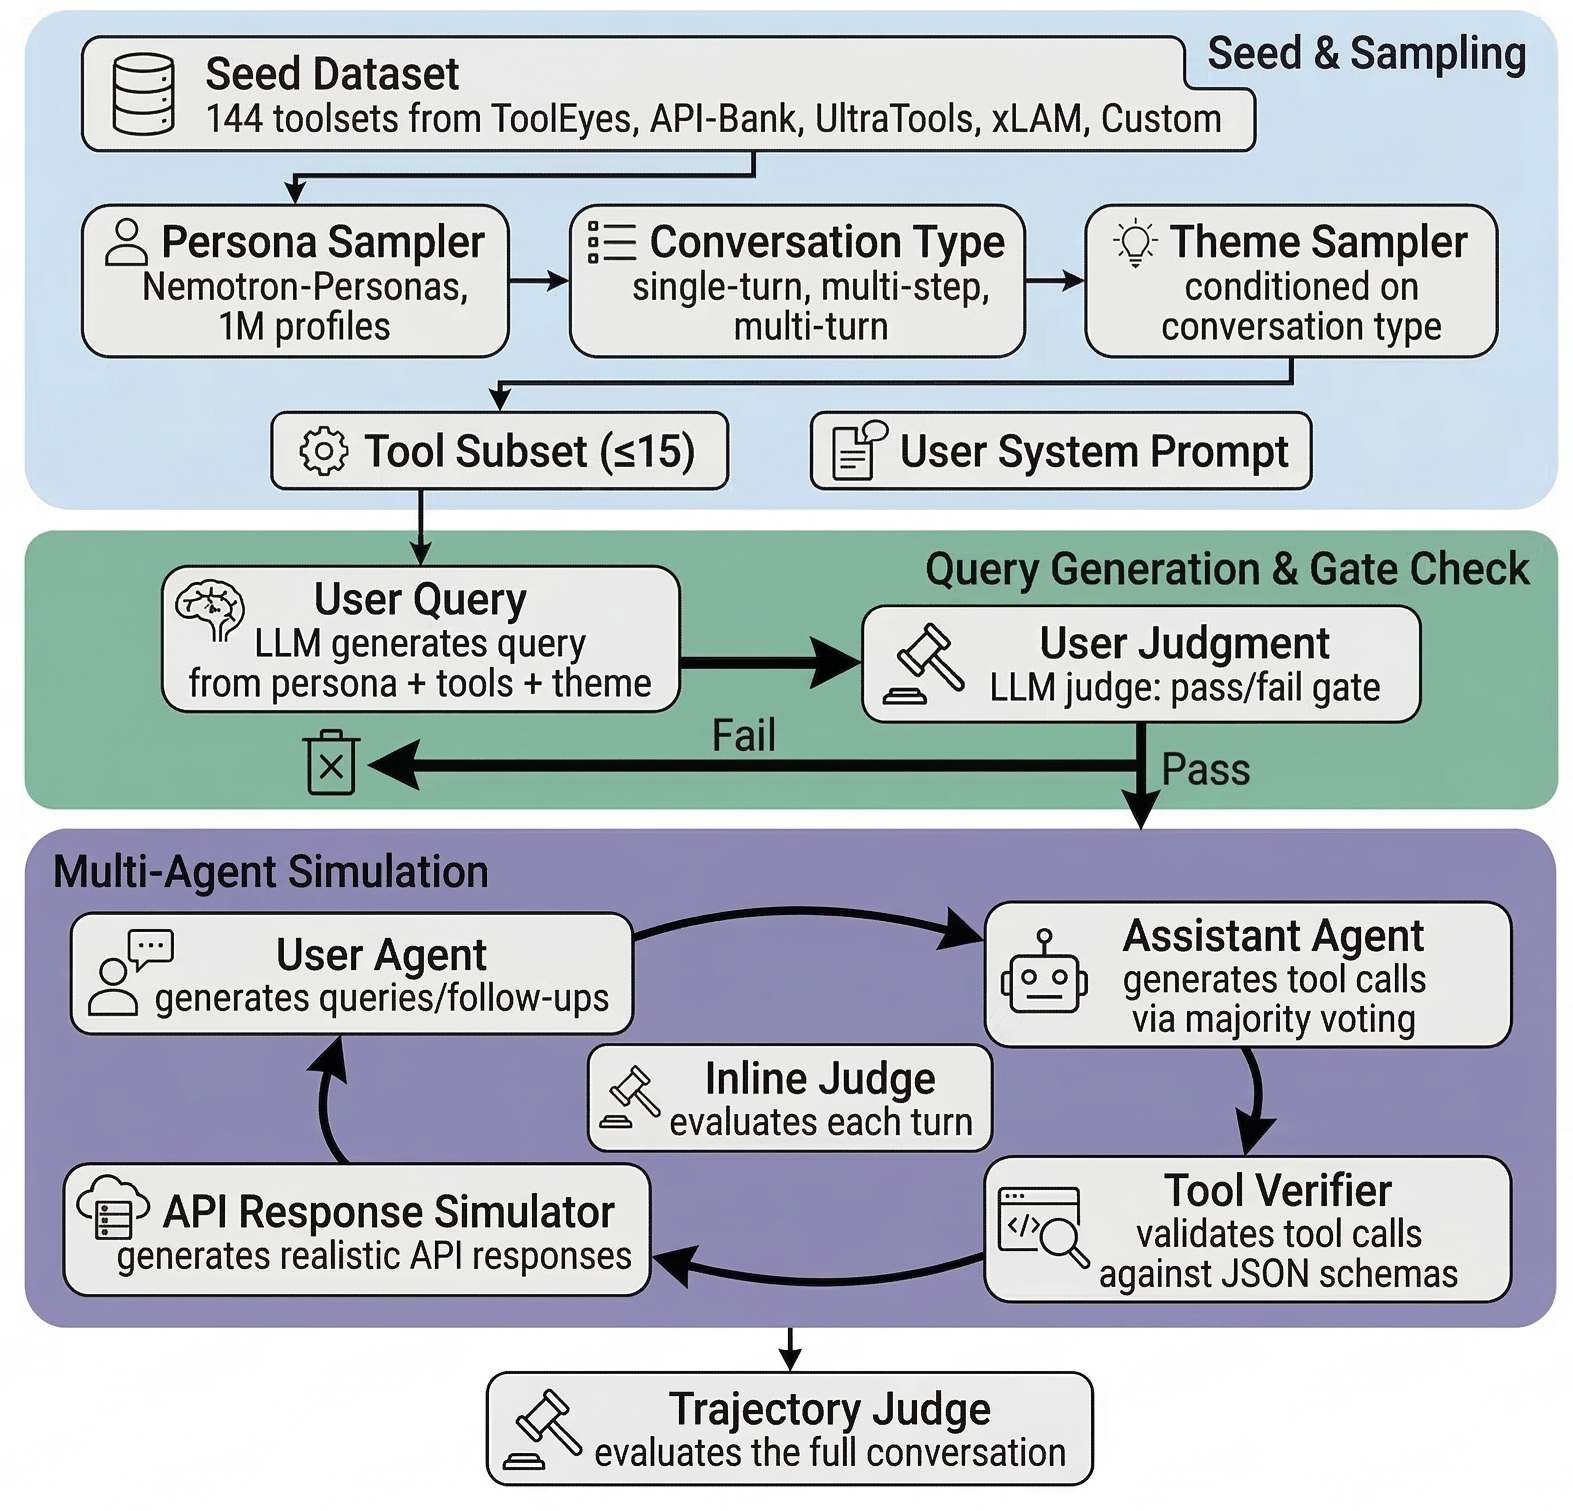
\includegraphics[width=0.5\linewidth]{figures/broad_conversational_tool_use-new.png}
% change the image to match template
\caption{Overview of the pipeline for general-purpose tool-calling data used in \ourmodel.}

\label{fig:broad_conversational_tool_use_data_generation_pipeline}
\end{figure}

% A comparison of the scale of SFT data used in model training compared to \texttt{\nanomodel} is shown in Table \ref{tab:conversational_tool_use_data_size}.
% \begin{table}[!t]
% \centering
% \begin{tabular}{lcc}
% \hline
% \textbf{Model} & \textbf{Number of Domains} & \textbf{Number of Conversations} \\ \hline
% \nanomodel & 5 & 15588 \\
% \ourmodel & 838 & 279116 \\ \hline
% \end{tabular}
% \caption{Size of conversational tool-use data used in SFT for \nanomodel vs \ourmodel. Using our synthetic data generation pipeline, we greatly increase the diversity and scale of the data by increasing the number of domains and conversations.}
% \label{tab:conversational_tool_use_data_size}
% \end{table}
% % 

% We generate synthetic multi-turn trajectories to demonstrate conversational tool use. The generation of these trajectories involves a user that is given a task to accomplish, an agent that is instructed to help the user accomplish their task, and a tool execution environment, each of which is simulated by a language model. To limit the trajectories in the SFT training data to ones in which the actions of all of these entities are consistent with their goals, we employ a language model as a judge to evaluate the trajectories, and filter out trajectories for which the judge considers an action of an entity to be inconsistent with its goals. We use Qwen3-235B-A22B-Thinking-2507 \citep{yang2025qwen3technicalreport}, Qwen3-32B \citep{yang2025qwen3technicalreport}, GPT-OSS-120b \citep{openai2025gptoss120bgptoss20bmodel}, and Qwen3-235B-A22B-Instruct-2507 \citep{yang2025qwen3technicalreport} to generate data in this synthetic tool use trajectory generation pipeline.

% \subsubsection{Data Filtering}
% We apply the same filtering process as Nemotron Nano v3.

\subsubsection{SFT Data Blend}
Our general stage 1 SFT data blend can be found in Figure \ref{fig:sft_blend} (all datasets not listed make up less than 1\% of the blend). We train on over 7M total samples. In stage 2, we use 85\% of the stage 1 blend and augments it with 256K and 512K-token long-context data. Compared to \nanomodel, we  significantly increased the volume and diversity of agentic tasks, and allocate it a much larger proportion of our blend.

\begin{figure}[t]
    \centering
    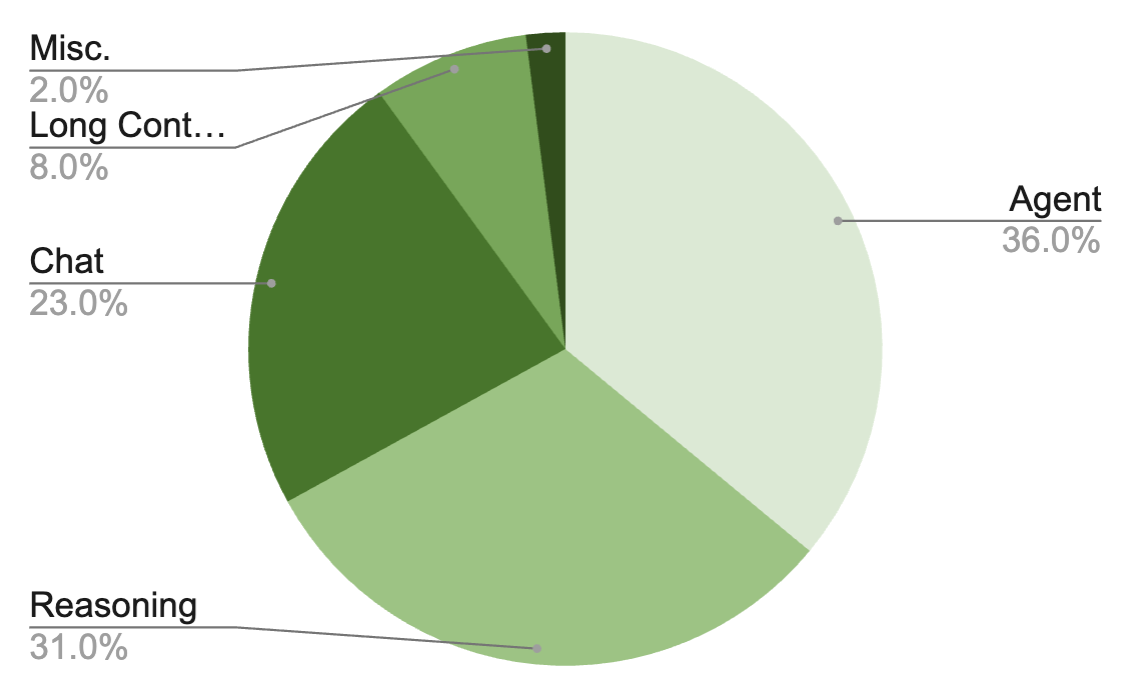
\includegraphics[width=10cm]{figures/super_sft_blend.jpg}
    \caption{SFT data blend for \ourmodel. }
    \label{fig:sft_blend}
\end{figure}


\subsubsection{Reasoning Control}

\ourmodel is trained for three reasoning modes: reasoning-off, regular and low-effort. The low-effort reasoning mode is a new addition.
The regular and low-effort reasoning modes have the option to be used in conjunction with inference-time budget control \citep{nvidia2025nemotronhfamilyaccurateefficient}.
These combinations of controls provide flexibilities that cover the entire spectrum of accuracy-efficiency trade-off to meet customers' needs in various application scenarios.

The low-effort reasoning mode is introduced during the SFT stage by adding training samples generated by GPT-OSS-120B in its low-effort mode \citep{du2025nemotron}.
These low-effort training samples cover the tasks of math reasoning, STEM question answering and instruction following, and represent 2\% of the overall SFT data by sample count.
The low-effort mode is later optimized during the RL stages to be discussed in the next section.

The SFT recipe for reasoning-off mode and for inference-time budget control is similar to \cite{nvidia2025nemotron3nanoopen} with a few differences.
We strip the reasoning traces from a random 3\% samples for reasoning-off mode.
After the main SFT stage, we add a short semi-on-policy SFT stage of 350 steps for inference-time budget control, where we collect roll-outs from the model and truncate 12\% of reasoning traces to random reasoning budgets.

%\ourmodel allows for three different forms of reasoning control: reasoning on/off control, token budget control, and a new reasoning low mode. To enable reasoning on/off control and budget control, we follow the same approach as \citep{nvidia2025nemotron3nanoopen}. To enable a reasoning low mode, we add low reasoning budget traces from GPT-OSS in the SFT stage, and conduct RL training to further improve the reasoning low mode performance.


% \subsection{Reinforcement Learning}
% \label{subsec:RL}
% The RL phase of \ourmodel post-training comprises three stages as shows in Figure \ref{fig:posttraining_stages}: Stage (1) multi-environment RLVR \ref{subsub:rlvr}, Stage (2) reinforcement learning for end-to-end software engineering tasks (SWE-RL) \ref{subsub:swerl}, and Stage 3 RLHF. \ref{subsec:RLHF}
% We detail each stage along with the training algorithm and systems setup below.

% Multi-environment RLVR is the primary stage and trains on the full set of environments simultaneously. We use this unified setup to keep RL updates informed by the full environment mix and to prevent accuracy drops across all tasks throughout the run.

% We handle end-to-end SWE-RL separately as the second stage since it has very different systems characteristics from the rest of the environments. SWE-RL rollouts take substantially longer to generate and often require longer context lengths, which makes them a throughput bottleneck when trained alongside the other environments. We therefore run RL for the SWE tasks as a separate stage using settings tuned for long-horizon, long-context trajectories. 

% We finally run RLHF as a distinct stage to improve the model behavior and interaction quality.

% \subsubsection{Multi environment Reinforcement Learning from Verifiable Rewards}
% \label{subsec:RLVR}

\subsection{Reinforcement Learning}
\label{subsec:RL}
The RL phase of \ourmodel post-training consists of three stages followed by an MTP healing stage as shown in Figure~\ref{fig:posttraining_stages}:
\begin{itemize}
    \item[] --- \textbf{Stage 1: Multi-environment RL from Verifiable Rewards} (\S\ref{subsub:rlvr}). This is the primary training stage, where we optimize \ourmodel jointly across the full set of environments. Training in a unified mixture keeps each RL update informed by the complete environment distribution and helps prevent regressions on individual tasks over the course of training.
    \item[] --- \textbf{Stage 2: SWE-RL for end-to-end software engineering tasks} (\S\ref{subsub:swerl}). We run SWE-RL as a separate stage because SWE rollouts are substantially slower to generate and typically require longer context lengths, creating a throughput bottleneck when co-trained with shorter-horizon environments. Isolating this stage allows us to tune rollout and batching settings for long-horizon, long-context trajectories.
    \item[] --- \textbf{Stage 3: RLHF} (\S\ref{subsec:RLHF}). We finally apply RLHF as a distinct stage to improve instruction-following behavior, robustness, and overall interaction quality.
    \item[] --- \textbf{Stage 4: MTP Healing}. In this stage we train the MTP heads and keep rest of the weights frozen. We re-use the prompts from RLVR, and train the MTP head using the negative log likelihood loss similar to SFT on the generated responses. We find this stage significantly improves MTP accuracy.
\end{itemize}

We describe these stages below including the training algorithm, data and systems setup.



\subsubsection{Stage 1: Multi-environment RL from Verifiable Rewards}
\label{subsub:rlvr}

We employ a unified RLVR strategy similar to \nanomodel, but significantly scale the number of environments. We find that training on all environments simultaneously yields stable gains, whereas single-environment training leads to severe regressions on other benchmarks.

Our RLVR setting contains 21 environments covering diverse domains, including math, code, STEM, safety, chat, instruction following, long context capabilities, puzzles, and various agentic tasks. For data mixture and curriculum, we adopt an approach similar to \nanomodel: we filter out prompts where the SFT model consistently provides correct answers, then sort the remaining samples via a difficulty-based curriculum. Further details of this methodology are available in \nanomodel.

\paragraph{Low-effort Reasoning}
During the multi-environmental RL stages, we convert a subset of the prompts to be in the low-effort mode. For each low-effort prompt, the reward for a roll-out is adjusted as a function of both correctness and the number of generated tokens. The low-effort prompt mix starts with subsets of Math, STEM QA and competitive coding prompts, in total representing 2\% of all RL prompts being in low-effort mode, and is later reduced to subsets of Math and STEM QA, representing just 1\% of RL prompts. For Math and STEM QA, we randomly sample a subset. For competitive coding, we have a set of coding problems that have been withheld from SFT data and we only sample from this withheld set for low-effort coding prompts. Empirical results suggest that this data strategy provides sufficient generalization and the low-effort mode is improved across a wide set of benchmarks during the course of multi-environmental RL.


\subsubsection*{RLVR Data}
We scale up our RL data significantly compared to \nanomodel. We describe the RL datasets we used in our multi environment RL below. The majority of the RL training environments are open sourced in Nemo Gym \citep{nemo-gym}. In total, we train on 21 environments and 37 different RL datasets.

\begin{itemize}
    \item[] --- \textbf{Math.} We use the same competitive math problems as \nanomodel. For this dataset, we train both with and without a Python execution tool. We also introduce a new environment for formal proof verification.
    \item[] --- \textbf{Code.} We train on competition-style code data from \nanomodel and \citet{wang2025nemotroncascadescalingcascadedreinforcement}. We also train on single-step patch generation for software engineering tasks to prepare for end-to-end RL in the next stage.
    \item[] --- \textbf{STEM.} We include the STEM datasets from \nanomodel and add newly curated, more challenging scientific problems.
    \item[] --- \textbf{Instruction Following.} We augment the instruction-following data from \nanomodel with a new multi-challenge dataset. In this setting, the agent must follow complex user instructions, with rewards computed from a predetermined rubric.
    \item[] --- \textbf{Safety.} We add two environments: one targeting reduced over-refusals on safety-related prompts, and one improving robustness to jailbreaks. For jailbreaks, seed prompts come from our SFT data; to surface harder attacks during RL, we apply an iterative attack pipeline following PAIR \citep{chao2024jailbreakingblackboxlarge}, attacking an early SFT-only checkpoint and collecting modified prompts with high attack success rates.
    \item[] --- \textbf{Long Context.} We use the same long-context environment introduced in \nanomodel.
    \item[] --- \textbf{Agentic Tool Use.} Beyond the tool-use environments from \nanomodel, we add new environments focused on conversational tool use and terminal use.
    \item[] --- \textbf{Reasoning Gym.} We train with Reasoning Gym \citep{stojanovski2025reasoning}, enabling learning over a diverse suite of reasoning tasks.
\end{itemize}

% \textbf{Math. } We train on the same competitive math problems as \nanomodel. When training \ourmodel on this dataset, we enable training both with and without a python execution tool. In addition, we create a new environment for formal proof verification.

% \textbf{Code. } We train on the competition code data from \nanomodel and \citet{wang2025nemotroncascadescalingcascadedreinforcement}.

% \textbf{Stem. } We train on the datasets from \nanomodel as well as newly curated and more difficult scientific problems.

% \textbf{Instruction Following. } We augment the instruction following datasets from \nanomodel with a new multi-challenge style dataset. In this dataset, the agent must must follow complex instructions given by the user and reward is based on a predetermined rubric.

% \textbf{Safety. } We introduce two additional environments when training \ourmodel. The first one focuses on mitigating overrefusals in responses to safety related prompts and the second one focuses on providing robustness against jailbreak attacks. For the jailbreak environment, the seed jailbreak prompts are collected from our SFT dataset. However, to ensure that we engage with challenging jailbreak prompts during RL, we use an iterative attack pipeline following the PAIR method \cite{chao2024jailbreakingblackboxlarge}, to directly attack an early SFT-only checkpoint and collect modified prompts that show a high attack success rate. 

% \textbf{Long Context. } We use the same long context environment developed in \nanomodel.

% \textbf{Agentic Tool Use. } In addition to the environments from \nanomodel, we introduce several new environments focused on conversational tool use and terminal use.

% \textbf{Reasoning Gym. } We train \ourmodel using Reasoning Gym \citep{stojanovski2025reasoning}, allowing our model to learn from a diverse set of reasoning tasks.

\subsubsection{Stage 2: End-to-end RL for Software Engineering}
\label{subsub:swerl}
In the SWE-RL stage, we improve the model's ability to autonomously solve GitHub issues under diverse harnesses. Each rollout launches an Apptainer container with the target repository, runs an OpenHands agent loop to produce a code patch, and evaluates it against ground-truth tests for a binary reward. For tool diversity, we implemented OpenCode and Codex agent classes within OpenHands that match the tool formats of Claude Code and Codex CLI, reusing a single harness while varying tools and prompts at training time. This multi-harness training improves the model's generalization and performance across all target harnesses at inference time.

\subsubsection{Stage 3: Reinforcement Learning from Human Feedback}
\label{subsec:RLHF}
We follow a similar approach to \nanomodel for RLHF, training a large GenRM model to provide supervision during RL. Rather than using a vanilla GenRM, we train a principle following GenRM as in \citet{wang2025rlbff}. These principles allow us to guide \ourmodel's behavior on important domains like identity and safety related topics. Similar to \nanomodel, we use \texttt{Qwen3-235B-A22B-Thinking-2507} as the initialization for training the GenRM. 

To train the GenRM we use the Helpsteer 3 dataset \citep{Wang2025HelpSteer3Preference}, commercially friendly subsets of the lmarena-140k dataset \citep{chiang2024chatbot}, and some more recently collected human preference data. Unlike \nanomodel, we train using our GenRM throughout our multi environment RL stage and also perform a separate RLHF-only stage at the end of post training.


\subsubsection{Algorithm}
We use an asynchronous GRPO setup in which training and inference are decoupled across separate GPU devices. Inference workers continuously generate trajectories, which are stored in a rollout buffer. Once enough trajectories are collected to form a batch, the batch is sent to the training engine for a model update. We push the updated weights to the inference workers as soon as a new model version is available. Because weight updates can happen mid-rollout, a single trajectory may contain tokens produced by different model versions. We do not recompute the KV cache after updating the model weights on the inference workers. To avoid excessive policy lag, which may result in accuracy degradation, we restrict the inference workers to be at most one step behind the latest model version.

To stabilize the training and minimize off-policy effects caused by the training-inference mismatch and policy lag, we mask the importance sampling ratio computed from the training and inference logprobs \citep{Shao2024DeepSeekMath, team2025every, yao2025offpolicy}.

In multi-environment RLVR, we sample 256 prompts per step and generate 16 responses per prompt. We train with a batch size of 4096, which corresponds to a single gradient update per rollout. We begin training with a maximum generation length of 49K tokens and later increase it to 64K.

\textbf{Agentic RL - PivotRL:}
Post-training for long-horizon agentic capabilities has a tension between efficiency and accuracy. By long-horizon, we mean tasks that require many turns of interaction with an environment, such as conversational tool use, code editing, terminal interaction, and web search. SFT is cheap and simple for this task, but it often degrades performance outside of the target domain (OOD). End-to-end RL avoids that outcome to a large part, but it is costly because every update requires online interactive rollouts in complex environments. To address this, during the post-training of Super, we adopt PivotRL~\citep{yi2026pivotrl}. 

PivotRL is an assistant-turn-level RL method that addresses this tradeoff by reusing offline SFT expert trajectories during RL. It focuses training on informative turns  (called "pivots") within those SFT traces, where the policy has uncertainty over the next action, and it uses a domain-appropriate reward to match the policy's action to the expert action, so the model gets credit for similar actions rather than the exact expert action. We notice that this method greatly improves the efficiency of our agentic RL, without facing the OOD degradation issues of SFT.

We apply PivotRL for all agentic domains: including for Agentic Programming, Search, Terminal Use, and Conversational Tool Use. We will have a manuscript with more details soon.

\subsubsection{Infrastructure}
RL at the frontier of model post-training is currently defined by scaling up to an increasing diversity of tasks or environments designed for the model to learn increasingly general capabilities. Scaling RL to many environments requires a high-performance, extensible, and standardized interface for coordinating between rollouts and training. To address the scaling performance and extensibility challenges using one standard framework, we adopt NeMo Gym \citep{nemo-gym} and NeMo RL \citep{nemo-rl} for enabling large-scale RL on many different environments/verifiers.

NeMo Gym is based on the abstraction of servers. There are three core varieties of servers in Gym: (1) agents, (2) models, and (3) resources. An agent server implements the rollout kernel of a RL environment. A model server wraps an inference engine such as vLLM \citep{kwon2023efficientmemorymanagementlarge} to provide a prompt-response API, and also carefully preserves token and inference log-prob data and metadata required for RL. A resource server provides a verification API for computing rewards from a given rollout.

Our Nemotron Super 3 RLVR experiments were all based on an integrated infrastructure of NeMo RL and NeMo Gym: NeMo RL acts as the RL training loop controller, using Megatron-Core \citep{shoeybi2020megatronlmtrainingmultibillionparameter} for model training at scale, and routing all rollouts through NeMo Gym and vLLM.

NeMo RL and NeMo Gym use ray for orchestration and resource management and deploy the ray cluster on SLURM. Megatron training workers, vLLM generation workers, Gym environments and judge models are all scheduled onto a single ray cluster.

\textbf{Async RL Infrastructure: } 
All RL stages used asynchronous RL, where generation can happen independently of training which improves training efficiency by trading off how on-policy the rollouts are. The trainings used one-step off policy where each training step was earmarked for a future training step so there were no wasted rollouts. Training and generation were not collocated which simplifies deployment and avoids having to orchestrate complex memory management between the async training and generation workers.

All asynchronous RL runs also used in-flight weight updates \citep{piche2025pipelinerl} where training can update generation worker weights without waiting for the remaining ongoing rollouts to finish. The result is a single rollout can have tokens and log probabilities from differently aged policies. Enabling in-flight weight updates is critical for speeding up asynchronous RL training. We did not recompute the KV cache after in-flight weight updates.

\textbf{Resiliency: }
As we scaled up to 1k GPUs, we encountered several issues that caused intermittent failures that were not observed in smaller job shapes. These issues fell into two categories (1) hardware related and (2) software related.

We observed several hardware issues that required full restart of the job, so several optimizations were also made to improve startup time by (1) parallelizing all initialization (2) prefetching all virtual environments and binaries (3) utilize caching in upstream repos like vLLM and flashinfer.

Parallel initialization exacerbated latent race conditions with port bindings in the post-training software stack, which became a significant failure point. Several components of the post-training software required ports: (1) Ray control plane (2) vLLM workers and OpenAI servers (3) TCP rendezvous (4) NeMo Gym servers. Due to the high number of processes needing ports on a node, we hit port conflict frequently at 1K GPU scale that were all time-of-check to time-of-use (TOCTOU) race conditions. The pattern we observed was that a component would check if a port was available without claiming it exclusively, and by the time it (or another process it notified) attempted to bind, another process had already claimed the port.


\textbf{SWE-RL Infrastructure: }
Training a model on software engineering tasks requires a gym environment that can execute hundreds of concurrent agent-codebase interactions, each within an isolated sandbox, and return a reward signal derived from real test execution. In the SWE-RL environment in Nemo-Gym, each rollout launches an Apptainer container with the target repository, runs the OpenHands agent loop to produce a code patch, and runs the ground-truth tests to compute a binary reward. Rollouts are distributed across nodes using Ray with a \texttt{SPREAD} scheduling strategy. Below we describe the key components of this environment.

\begin{itemize}
    \item \textbf{Container Execution with Apptainer.} The absence of root access on our cluster restricts the use of Docker for container isolation. Instead, we use Apptainer (formerly Singularity) to run each SWE task instance in a pre-built container image (\texttt{.sif} files), providing filesystem isolation via a writable tmpfs overlay while sharing the host kernel.

    \item \textbf{OpenHands Agent Loop.} The agent loop is executed by a modified version of OpenHands, managing the full lifecycle of each interaction: initializing the runtime, presenting the problem statement, running the agent's step loop upto a configurable turn limit, extracting the git patch, and cleaning up. The agent interacts with the repository workspace through bash commands and file operations via a tmux-based session.

    \item \textbf{Memory Management.} Since Apptainer containers share host memory and processes (unlike Docker's cgroup isolation), runaway agent processes can cause OOM conditions affecting the entire node. We implemented a memory watchdog daemon that monitors the aggregate RSS of the tmux process tree and proactively kills processes inside panes when a configurable limit is exceeded, while keeping the tmux server alive for graceful recovery.

    \item \textbf{Command Blocklist.} The shared-kernel nature of Apptainer means an agent issuing \texttt{killall} or \texttt{pkill} could terminate training processes or vLLM servers on the same node. A regex-based command block list intercepts and blocks dangerous commands before execution, returning informative error messages with safer alternatives.

    \item \textbf{Harness Diversity.} To increase tool diversity during training without building separate harness integrations, we implemented OpenCode and Codex agent classes within OpenHands that match the tool input/output formats of their respective external harnesses (Claude Code and Codex CLI). Both agents plug into OpenHands' existing runtime and conversation memory, inheriting container management and observation handling. 

    \item \textbf{Serialization.} We replaced Python's standard \texttt{json} with \texttt{orjson} for serialization of HTTP payloads between the gym and the model server, as each trajectory turn carries prompt token IDs, generated token IDs, and log probabilities, resulting in large payloads that benefit from orjson's Rust-based implementation.
\end{itemize}


% \subsection{Reinforcement Learning from Human Feedback}
% \label{subsec:RLHF}
% We follow a similar approach to \nanomodel for RLHF, training a large GenRM model to provide supervision during RL. Rather than using a vanilla GenRM, we train a principle following GenRM as in \citet{wang2025rlbff}. These principles allow us to guide \ourmodel's behavior on important domains like identity and safety related topics. Similar to \nanomodel, we use \texttt{Qwen3-235B-A22B-Thinking-2507} as the initialization for training the GenRM. 

% To train the GenRM we use the Helpsteer 3 dataset \citep{Wang2025HelpSteer3Preference}, commercially friendly subsets of the lmarena-140k dataset \citep{chiang2024chatbot}, and some more recently collected human preference data. Unlike \nanomodel, we train using our GenRM throughout our multi environment RL stage and also perform a separate RLHF-only stage at the end of post training.


\subsection{Post-trained Model Evaluations}
\label{subsec:final_model_evals}

% \subsubsection{Evaluation Benchmarks}

\begin{table*}[!htp]
\centering
\small
\setlength{\tabcolsep}{7pt}
\renewcommand{\arraystretch}{1.15}
\begin{tabular}{l|c c c}
\toprule
\textbf{Benchmark} & \textbf{N-3-Super} & \textbf{Qwen3.5-122B-A10B} & \textbf{GPT-OSS-120B} \\
\midrule

\rowcolor{black!5}
\multicolumn{4}{l}{\textbf{General Knowledge}} \\
MMLU-Pro & 83.73 & 86.70 & 81.00 \\

\midrule
\rowcolor{black!5}
\multicolumn{4}{l}{\textbf{Reasoning}} \\
AIME25 (no tools) & 90.21 & 90.36 & 92.50  \\
HMMT Feb25 (no tools) & 93.67 & 91.40 & 90.00  \\
HMMT Feb25 (with tools) & 94.73 & 89.55 & -  \\
% AIME25 (with tools) &  &  &  \\
GPQA (no tools) & 79.23 & 86.60 & 80.10 \\
GPQA (with tools) & 82.70 & - & 80.09 \\
LiveCodeBench (v5 2024-07$\leftrightarrow$2024-12) & 81.19 & 78.93 & 88.00 \\
SciCode (subtask) & 42.05 & 42.00 & 39.00  \\
HLE (no tools) & 18.26 & 25.30 & 14.90  \\
HLE (with tools) & 22.82 & - & 19.0 \\
% MiniF2F pass@1 &  &  &  \\
% MiniF2F pass@32 &  &  &  \\

\midrule
\rowcolor{black!5}
\multicolumn{4}{l}{\textbf{Agentic}} \\
Terminal Bench (hard subset) & 25.78 & 26.80 & 24.00 \\
Terminal Bench Core 2.0 & 31.00 & 37.50 & 18.70 \\
SWE-Bench (OpenHands) & 60.47 & 66.40 & 41.9 \\
SWE-Bench (OpenCode) & 59.20 & 67.40 & - \\
SWE-Bench (Codex) & 53.73 & 61.20 & - \\
SWE-Bench Multilingual (OpenHands) & 45.78 & - & 30.80 \\
\textbf{TauBench V2} &  &  &  \\
\quad Airline & 56.25 & 66.0 & 49.2  \\
\quad Retail & 62.83 & 62.6 & 67.80 \\
\quad Telecom & 64.36 & 95.00 & 66.00 \\
\quad Average & 61.15 & 74.53 & 61.0 \\
BrowseComp with Search& 31.28 & - & 33.89 \\
BIRD Bench & 41.80 & - & 38.25 \\

\midrule
\rowcolor{black!5}
\multicolumn{4}{l}{\textbf{Chat \& Instruction Following}} \\
IFBench (prompt) & 72.56 & 73.77 & 68.32 \\
Scale AI Multi-Challenge & 55.23 & 61.50 & 58.29 \\
% Arena-Hard-V2 (Hard Prompt) &  &  &  \\
% Arena-Hard-V2 (Creative Writing) &  &  &  \\
Arena-Hard-V2 & 73.88 & 75.15 & 90.26 \\

\midrule
\rowcolor{black!5}
\multicolumn{4}{l}{\textbf{Long Context}} \\
AA-LCR & 58.31 & 66.90 & 51.00 \\
RULER 256k & 96.83 & 96.74 & 52.30 \\
RULER 512k & 95.22 & 95.95 & 46.70 \\
RULER 1M & 91.64 & 91.33 & 22.30 \\

\midrule
\rowcolor{black!5}
\multicolumn{4}{l}{\textbf{Multilingual}} \\
MMLU-ProX (avg over langs) & 79.36 & 85.06 & 76.59 \\
WMT24++ (en$\rightarrow$xx) & 86.67 & 87.84 & 88.89 \\

\bottomrule
\end{tabular}

\caption{
Evaluation suite for \ourmodel. We compare against \textsc{Qwen-3.5-122B-A10B} and \textsc{GPT-OSS-120B}.
% (Values omitted in this template; to be filled with final scores.)
}
\label{tab:super_comparison}
\end{table*}

We evaluate \ourmodel on the same broad benchmark suite and evaluation stack as \nanomodel\citep{nvidia2025nemotron3nanoopen}, covering general knowledge, reasoning, agentic, instruction following, long-context, and multilingual capability. All evaluation results were collected via Nemo Evaluator SDK\footnote{\url{https://github.com/NVIDIA-NeMo/Evaluator}} and for most benchmarks, the Nemo Skills Harness\footnote{\url{https://github.com/NVIDIA-NeMo/Skills}}. For reproducibility purposes, the open source container on Nemo Skills packaged via NVIDIA's Nemo Evaluator SDK used for evaluations can be found here\footnote{\url{https://catalog.ngc.nvidia.com/orgs/nvidia/teams/eval-factory/containers/nemo_skills}}. In addition to Nemo Skills, the evaluations also used dedicated open-source packaged containers for Tau-2 Bench (default prompt), Terminal Bench Hard (48 tasks), ScaleAI Multi Challenge Multi-turn Instruction Following, Ruler. More details on the evaluation settings can be found in the Nemo Evaluator SDK configs folder\footnote{\url{https://github.com/NVIDIA-NeMo/Evaluator/tree/main/packages/nemo-evaluator-launcher/examples/nemotron/nemotron-3-super}}. The following benchmarks are not onboarded yet in our open source tools and for these we used either their official open source implementation or otherwise an internal scaffolding that we plan to open source in the future: SWE Bench Verified (OpenHands), SWE Bench Multilingual (OpenHands), BrowseComp with Search (internal implementation, with Serp API), Terminal Bench Core 2.0 (Harbor).

\paragraph{Reasoning Capabilities.}
We report results on \textsc{AIME 25}, \textsc{HMMT Feb 25}, \textsc{GPQA} \citep{rein2023gpqa}, \textsc{LiveCodeBench v5} \citep{jain2024livecodebench}, \textsc{SciCode} \citep{tian2024scicoderesearchcodingbenchmark}, and \textsc{HLE} \citep{phan2025humanitysexam}. Across all benchmarks \ourmodel is competitive with \texttt{GPT-OSS-120B}, while lagging behind \texttt{Qwen-3.5-122B} slightly.

\paragraph{Agentic capabilities.}
 We report results on \textsc{TerminalBench} (the hard subset and the v2 set),
\textsc{SWE-Bench} (OpenHands, OpenCode, Codex, and the Multilingual set) \citep{jimenez2023swe}, \textsc{TauBench V2} (Airline, Retail, Telecom; and their average) \citep{barres2025tau},
and \textsc{BrowseComp} \citep{wei2025browsecomp}. For Browsecomp, our harness takes strong inspiration from the browser tool released with GPT OSS. \citep{openai2025gptoss120bgptoss20bmodel}, and we do not evaluate with any context management strategies. For SQL we evaluate on the BIRD benchmark \cite{li2023bird} dev set (1,534 samples, SQLite, execution accuracy). Across all agentic benchmarks, \ourmodel outperforms or is competitve with GPT-OSS 120B and is competitive to Qwen 3.5 122B on some harnesses. 

 

% The Nemotron Super model achieves 41.80\% EX (5-run average), outperforming GPT-OSS-120B \cite{agarwal2025gpt} at 38.25\% EX under identical NeMo Skills evaluation conditions. Absolute EX scores are not directly comparable to BIRD leaderboard results, which use optimized schema representations; all models here share the same standardized prompt for fair comparison.

\paragraph{Chat and Instruction Following Capabilities.}
We report results on \textsc{IFBench}, \textsc{Multi-Challenge}, \textsc{Arena-Hard V2} \citep{li2024wildchat}. Across all benchmarks \ourmodel is competitive with the baseline models.

\paragraph{Long Context Capabilities.}
We report results on \textsc{Ruler} \citep{hsieh2024ruler} using 100 samples per task and \textsc{AALCR}. 
% \ourmodel achieves competitive performance in this category, demonstrating its efficacy in long context scenarios.

\paragraph{Multilingual Capabilities.}
We measure multilingual capability on 
\textsc{MMLU-ProX} \citep{xuan2025mmlu} and \textsc{WMT24++} en$\rightarrow$xx \citep{deutsch2025wmt24++}. \ourmodel matches or outperforms the baseline models on both bencharks.

For comparison with \textsc{GPT-OSS-120B} and \textsc{Qwen-3.5-122B-A10B}, we use officially reported numbers
whenever available; when not available, we follow the \nanomodel report \citep{nvidia2025nemotron3nanoopen} procedure of either sourcing values
from reputable public aggregators (when consistent with the official protocol) or computing scores
ourselves using the official evaluation settings.

